\section{Développement}
Toutes les parties nécessaires pour concevoir un agent conversationnel basé sur une architecture neurale existent présentement. Certaines techniques se sont démarquées au fil des études. Un survol succinct des techniques les plus prometteuses est fait, de façon à ce qu'il soit possible de joindre ces dernières ensemble ce qui permettrait d'en faire une implémentation réelle et complète. Les approches neurales les plus aux goûts du jour sont à favoriser et sont introduites dans cet article. Ces approches imitent la nature et correspondent, à ce jour, à la forme la plus répandue d'intelligence artificielle. Il ne reste qu'à les informatiser convenablement et à découvrir les bonnes configurations neurales dans le but de créer l'interface conversationnelle idéale. \\

\subsection{Traitement d'un intrant vocal}
La première étape de calcul au sein d’une architecture neurale destinée à comprendre et répondre à un utilisateur est justement de comprendre ce qu’il dit. Pour accomplir cette tâche, il est possible d’utiliser un réseau de neurones \gls{tc}-\gls{dnn}-\gls{bilstm}-\gls{dnn}, c’est-à-dire des convolutions temporelles (\gls{tc}) suivies de couches de neurones linéaires profondes (\gls{dnn}), d’un \gls{lstm} bidirectionnel (\gls{bilstm}) et puis d’un second \gls{dnn} \cite{acousticModeling}. Ainsi, cette architecture dépend d’un prétraitement du signal par un autre algorithme lequel est plus classique et permet de transformer le signal en un domaine de fréquences personnalisées. C’est ce prétraitement de l’information qui est introduit dans le réseau de neurones profonds, afin d’en analyser le sens et de le pouvoir convertir en états acoustiques, lesquels peuvent être convertis, cette fois, en texte littéraire. Cette architecture neurale, imagée à la \autoref{fig:tcDnnBlstmDnn}, obtient un \gls{wer} de retranscription de 3.47, ce qui est présentement le \gls{sota} sur le jeu de données du problème du \gls{wsj} eval’92.

\begin{figure*}
  \centering
  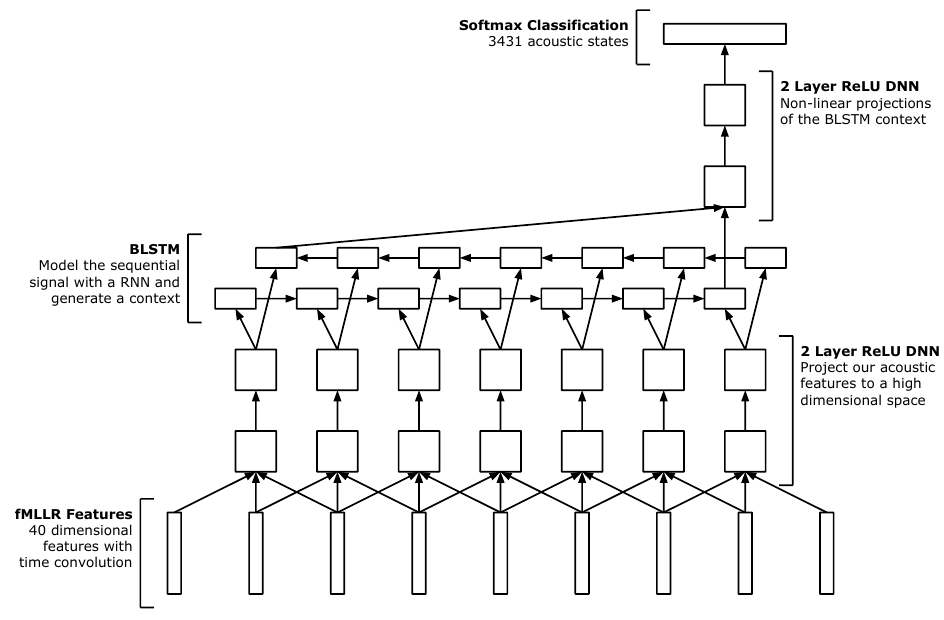
\includegraphics[width=\textwidth]{tcDnnBlstmDnn}
  \caption{L’architecture neurale \gls{tc}-\gls{dnn}-\gls{bilstm}-\gls{dnn} permet d’écouter le signal sonore à l’aide des données audio extraites en \gls{fmllr}. Ainsi, un \gls{dnn} suivi d’un \gls{bilstm} peut analyser ce signal pour classifier le tout en états acoustiques, lesquels sont eux-mêmes repris par un algorithme classique qui permet de rassembler ces états en mots réels. Notons que cette architecture neurale peut être utilisée pour raffiner le signal des mots prononcés, ce qui peut être envoyé directement dans un réseau de neurones supérieur en tant que \textit{embedding}. [\citenum{acousticModeling}]}
  \label{fig:tcDnnBlstmDnn}
\end{figure*}

\subsection{Extraction des composantes de l'intrant et des sources d'information à analyser}
\label{devel:embedding}
Une fois que la requête de l'utilisateur est convertie sous une forme textuelle facilement manipulable par un ordinateur, il est possible, dès lors, d'utiliser un \textit{embedding} induit par l'étape précédente. Une autre approche consiste à reprendre cette sortie pour ensuite la fournir à une nouvelle structure qui se chargera d'aller extraire de nouvelles composantes qui aideront certainement à obtenir de meilleurs résultats pour la suite du processus. \\

À ce stade, nous devons comprendre que le signal est encore purement textuel et nous n'avons pour seule information qu'une décomposition des mots qui forment la demande reçue. Cependant, les langages sont formés de davantage de subtilités qu'un simple enchaînement de mots les uns après les autres. En effet, chaque mot joue un rôle précis dans la structure de la phrase et apporte une nuance particulière au contexte général de celle-ci ou encore du texte avec une plus faible portée. C'est exactement ce que les travaux de \cite{word2vec} visaient à faire. En 2013, ce groupe de chercheurs a fait la publication d'un article détaillant leur approche en comparant plusieurs modèles comprenant autant des approches classiques que des approches neurales. En plus de faire état de leurs travaux, ce groupe est aussi à l'origine d'outil qui est encore à ce jour considéré comme un incontournable: \texttt{word2vec}. \\

Malgré le fait que cet article porte sur les approches neurales, cet outil a plutôt prouvé que des modèles plus simplistes et classiques sont parfois plus appropriés. En ce qui concerne \texttt{word2vec}, ce dernier se fonde sur la combinaison de deux techniques nommées \gls{cbow} (\autoref{fig:cbow}) et \gls{skipgram} (\autoref{fig:skipgram}). Alors que le \gls{skipgram} se concentre à essayer de prédire le contexte environnant d'un mot donné, le \gls{cbow} cherchera plutôt à prédire la valeur considérée à partir de son environnement accordant ainsi plus d’importance à la structure des phrases plutôt qu’au contexte de son utilisation.\\

\begin{figure}[ht]
  \centering
  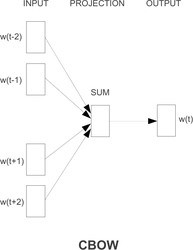
\includegraphics[width=\columnwidth, height=0.35\textheight, keepaspectratio]{cbow}
  \caption{Architecture de la méthode de prédiction \gls{cbow} [\citenum{word2vec}]}
  \label{fig:cbow}
\end{figure}

\begin{figure}[ht]
  \centering
  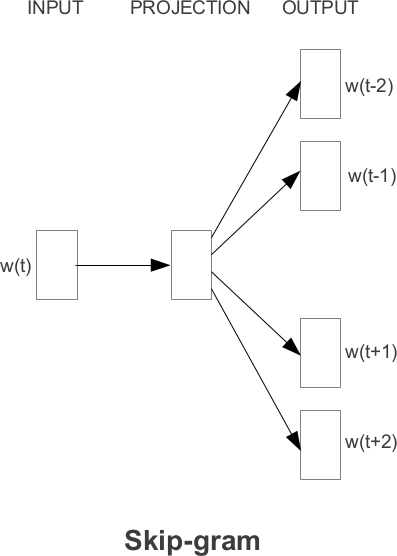
\includegraphics[width=\columnwidth, height=0.35\textheight, keepaspectratio]{skipgram}
  \caption{Architecture de la méthode de prédiction \gls{skipgram} [\citenum{word2vec}]}
  \label{fig:skipgram}
\end{figure}

En fournissant la requête reçue à cet outil, il est donc possible d'extraire les composantes sémantiques et syntaxiques sous-entendues dans cette dernière. Par la suite, ces nouvelles composantes seront combinées à celles déjà obtenues à l'étape précédente. En procédant avec cette seconde approche, un gain majeur est réalisé au niveau de la performance des étapes de modélisation subséquentes en raison de l'ajout de dimensionnalités qui fourniront beaucoup plus de flexibilité pour détecter les nuances du langage. À titre d'exemple, lorsqu'un utilisateur demandera à l'assistant si ce dernier peut lui indiquer l'horaire du cinéma le plus prêt de sa position, l'assistant devra comprendre la nuance que ce qui intéresse vraiment l'utilisateur est l'horaire et non pas l'évaluation booléenne de sa capacité à s'acquitter de cette tâche. Par contre, dans le cas où l'utilisateur demanderait à l'assistant si ce dernier peut le connecter à l'Internet, l'assistant devra dans ce cas faire l'évaluation de sa capacité et répondre par affirmation à ce cher utilisateur. \\

Mais qu'en est-il de nos sources d'informations? En fait, le processus entier bénéficiera qu'un travail similaire soit réalisé à ce niveau aussi. Pour ce faire, les alternatives suivantes s'offrent à nous. La première consistant encore une fois à utiliser \texttt{word2vec} et la seconde repose sur le même principe, mais à un niveau supérieur d'abstraction en considérant cette fois l'utilité de chacune des phrases dans le texte plutôt que de se concentrer sur le rôle de chaque mot dans chaque phrase \cite{inferSent}. De plus, il est possible d'utiliser les représentations neurales intermédiaires du réseau de neurones du système précédent dans le flot d'information afin d'y extraire des informations sur la personne qui parle provenant du contexte vocal plutôt que textuel. \\

En somme, toutes ces composantes ainsi dérivées pourront ensuite être fournies en entrée d'un réseau de neurones tel qu'un \gls{rnn} comme il est expliqué à section suivante. En effet, un \gls{rnn} peut lire des mots une fois les mots transformés en \textit{embedding}, ce qui est propice à une utilisation neurale de ces mots.

\subsection{Interpréter la requête et cibler le contenu d'intérêt pour y répondre}
\label{devel:qa}

Pour analyser les demandes de l'utilisateur, il faut les traduire en requêtes neurales pour ensuite rechercher dans le texte les passages intéressants. Cela est une étape importante à comprendre avant d'analyser davantage ce qui sera expliqué dans les prochaines sections. C'est l'une des choses que peuvent faire les mécanismes d'attention tels qu'introduits par \cite{attentionMechanism}. Ces mécanismes sont illustrés à la \autoref{fig:attn}. Son fonctionnement va comme suit. En premier lieu, le texte est lu séquentiellement en entrée (en bas à gauche). Ensuite, une requête est faite pour filtrer ce qui est lu et faire l'alignement d'attention (en bas à droite). Cette requête peut provenir d'un autre réseau de neurones, mais est ici elle-même générée dans un contexte de traduction automatique. La requête est donc de demander par quoi la phrase devrait débuter lors de ce début de traduction, ce que le décodeur (à droite) peut utiliser pour construire mot par mot une phrase traduite avec une requête à chaque nouveau mot, séquentiellement. Cette requête est à chaque étape comparée à toute l'information à filtrer par le mécanisme d'attention (au centre). C'est ainsi qu'un résultat est formulé par ce calcul du mécanisme d'attention en fonction de la requête demandée (en haut). Les auteurs soutiennent que les mécanismes d'attention sont à explorer plus en profondeur et que cela n'est que leur début. Une certaine exploration de ce mécanisme est faite par \cite{attentionBasedApproaches}. Dans ce papier, ils définissent, entre autres choses, un tel mécanisme comme étant un mini réseau de neurones dans un plus gros. Ce mini réseau de neurones sert à déterminer où porter de l'attention, et peut prendre des formes variées, tel qu'un réseau de neurones linéaire à deux couches, ou bien une comparaison par produit vectoriel de chaque élément à comparer à la requête, en tant que mesure de similarité entre la requête et les éléments d'information où rechercher. \\

\begin{figure*}
  \centering
  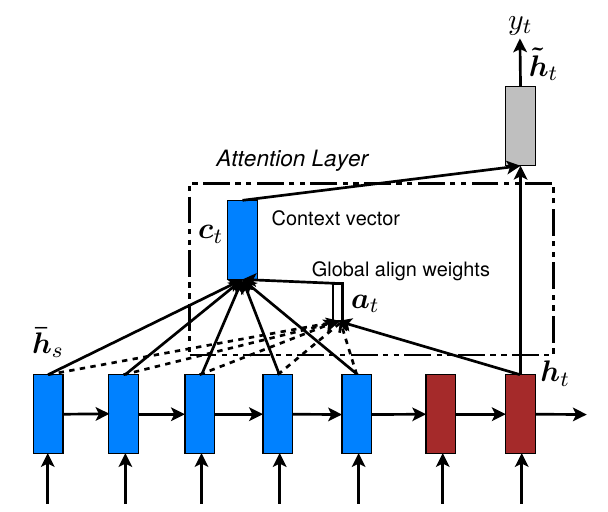
\includegraphics[width=\textwidth, height=0.4\textheight, keepaspectratio]{bahdanauAttentionMechanism2014}
  \caption{Mécanisme d'attention sous sa forme générale, tel qu'introduit par \cite{attentionMechanism} et ici raffinés par \cite{attentionBasedApproaches} dans cette figure.}
  \label{fig:attn}
\end{figure*}

Il est bien d'utiliser des mécanismes d'attention pour faire de la traduction automatique \cite{attentionMechanism}, mais il est tout aussi possible de les utiliser pour trouver dans du texte les passages intéressants en fonction d'une question? C'est ce que font \cite{squad\string:attentionOverAttention}, tout comme \cite{squad\string:coattention} sur le jeux de données du SQuAD \cite{squad}, les deux approches s'inspirant des travaux de \textbf{Google}, lesquels sont détaillés à la section suivante, \cite{readNcomprehend}. Les travaux de Cui et al. sont illustrés à la \autoref{fig:coAttn}.

\begin{figure*}
  \centering
  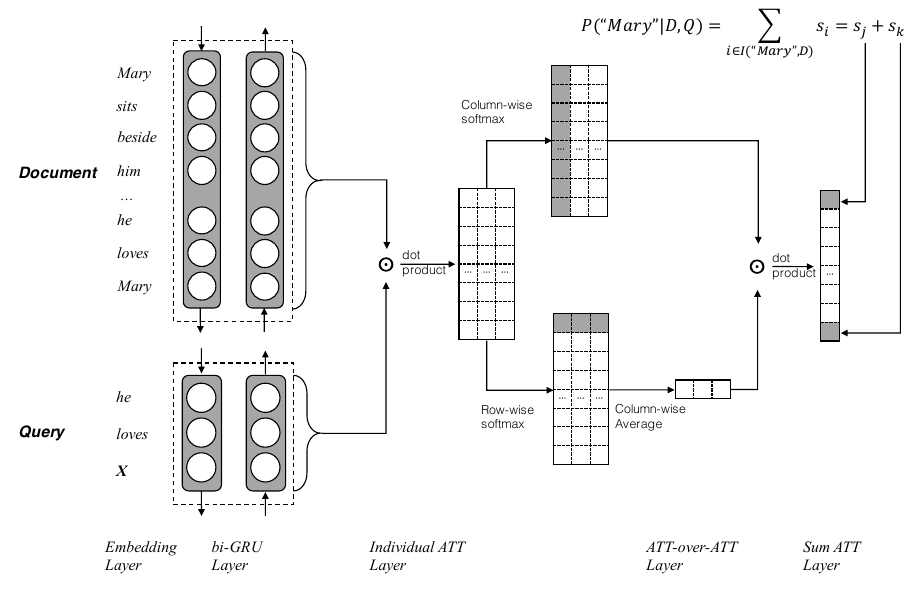
\includegraphics[width=\textwidth, height=0.4\textheight, keepaspectratio]{squadAttentionOverAttention}
  \caption{Réseaux de neurones profonds permettant d'analyser un document (en haut à gauche) en fonction d'une requête (en bas à gauche) pour produire une réponse avec l'information trouvée (à droite) \cite{squad\string:attentionOverAttention}.}
  \label{fig:coAttn}
\end{figure*}

\subsection{Formulation d'une réponse à partir de l'information d'intérêt retenue}

Bien qu’il est intéressant de trouver l’endroit où porter attention dans un corpus textuel, il est tout autant intéressant de savoir comment générer une réponse structurée et concise à l’utilisateur. Cela peut être fait en utilisant le \gls{hred} tel qu’introduit par \cite{chatbot\string:HRED}. En effet, \gls{hred} est une imbrication hiérarchique de réseaux de neurones récurrents. Un premier est utilisé afin d’encoder les phrases, un second est nécessaire afin de garder le contexte des réponses passées lesquelles ont déjà été traitées \footnote{Comme un suivi de la discussion dans une mémoire temporaire} et un troisième \gls{rnn} est mis à profit afin de décoder l’information en une réponse à l’utilisateur. En adaptant l'architecture neurale \gls{hred} de façon à lui donner des mécanismes d'attention tels que précédemment expliqués, il est possible de générer la réponse en retour de la requête attentionnelle à l’utilisateur. Ainsi, en ayant le contexte de la question que l'utilisateur pose ainsi que le contexte des documents à parcourir avec les mécanismes d’attention, il est possible de chercher dans le texte ce qu'il faut comme information, ce qui est envoyé au décodeur du \gls{hred} lequel peut répondre avec le nouveau contexte de l'information trouvée par la recherche effectuée. Ainsi, le premier \gls{rnn} du \gls{hred} qui encode l’information peut utiliser \texttt{word2vec} \cite{word2vec} directement, en plus de l'\textit{embedding} provenant de l’avant dernière couche de neurones du \gls{dnn} de la partie \gls{stt}. En plus de cela, il est possible d’utiliser \texttt{inferSent} de \textbf{Facebook} \cite{inferSent}, dont la sortie pourra être concaténée au signal de sortie du \gls{rnn} encodeur du \gls{hred}, en tant qu'\textit{embedding} supplémentaire au niveau des phrases plutôt qu’au niveau des mots comme expliqué à la \autoref{devel:embedding}. \\

Dans une amélioration plus récente de l’architecture \gls{hred} \cite{chatbot\string:LVHRED}, présentée à la \autoref{fig:lvHred}, il est possible d’utiliser une variable latente intermédiaire laquelle permet de faire le pont entre les réponses envoyées du décodeur vers l’utilisateur, en plus de réinjécter cette réponse dans l’encodeur qui écoute la réponse de l’utilisateur après lui avoir répondu une première fois. En retournant ainsi l'information du décodeur dans l’encodeur, le contexte se retrouve à être conservé d’une phrase à la prochaine et d'ainsi avoir un discours plus fluide tout en étant moins assujettis à des variations subites de sujet ou d'interprétation. D'autre part, ce passage d'information aura pour effet de renforcer la qualité de la requête attentionnelle laquelle peut être générée à la toute fin de l’encodeur du \gls{hred}. C'est à ce moment que le mécanisme d’attention décrit dans la \autoref{devel:qa} portant sur l’analyse de texte suite à des questions pourrait être inséré. Une fois la question posée par l’utilisateur et lue dans l’encodeur, le \gls{hred} peut bénéficier de cette question dans son \gls{rnn} intermédiaire, et ce, en tant que requête attentionnelle à passer directement au système attentionnel. Des travaux similaires ont été réalisés par \cite{readNcomprehend}, chez \textbf{Google}. Somme toutes, le \gls{hred} aura accès à la question de l’utilisateur et au corpus de texte dans lequel il peut maintenant cibler l’information pertinente.

\begin{figure*}
  \centering
  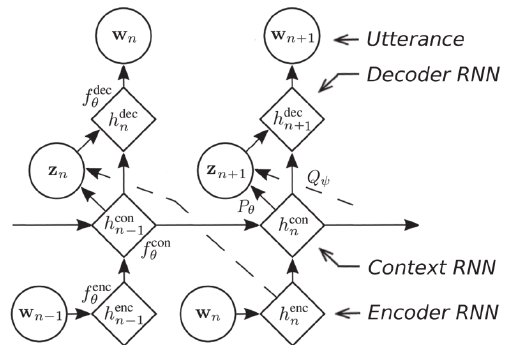
\includegraphics[width=\textwidth]{lvHred}
  \caption{L'architecture \gls{hred} améliorée avec une variable latente \cite{chatbot\string:LVHRED}}
  \label{fig:lvHred}
\end{figure*}

Étant donné la taille énorme du corpus textuel dans lequel le réseaux de neurones peut lire l’information \footnote{L’ensemble du texte sur Wikipédia par exemple}, il est possible d’appliquer un \texttt{MapReduce} \cite{DeanMapReduce} pour ainsi améliorer les performances de ce processus et réduire de façon importante le temps de réponse de notre assistant, ce qui est un aspect primordial à son déploiement et son adoption de la part de l'utilisateur. Cette technique procède de façon distribuée sur plusieurs centaines d’ordinateurs. Dans le cas présent, ceux-ci utiliseraient eux-même les implémentations de \texttt{word2vec} et de \texttt{inferSent} sur le corpus d'information, et cela en ayant en main la requête attentionnelle générée par le mécanisme d'attention, selon les principes de \texttt{MapReduce}. Cette partie, qui est distribuée et qui est surnommée, le lecteur impatient, est exposée à la \autoref{fig:teachingImpatientReader}. Il existe même une amélioration possible sur cet architecture neurale. Il est visible dans la figure que plusieurs itérations entre la requête et le système attentionnel est fait. Cela devrait être simplifié en une seule étape afin de réduire la complexité algorithmique de linéaire à constante en fonction de la longueur de la requête, en termes de nombre de mots. La recherche suivant la requête pouvant être distribuée, il devient donc très rapide d'accomplir le celle-ci, tout comme l'ensemble des opérations décrites aux sections précédentes.

\begin{figure*}
  \centering
  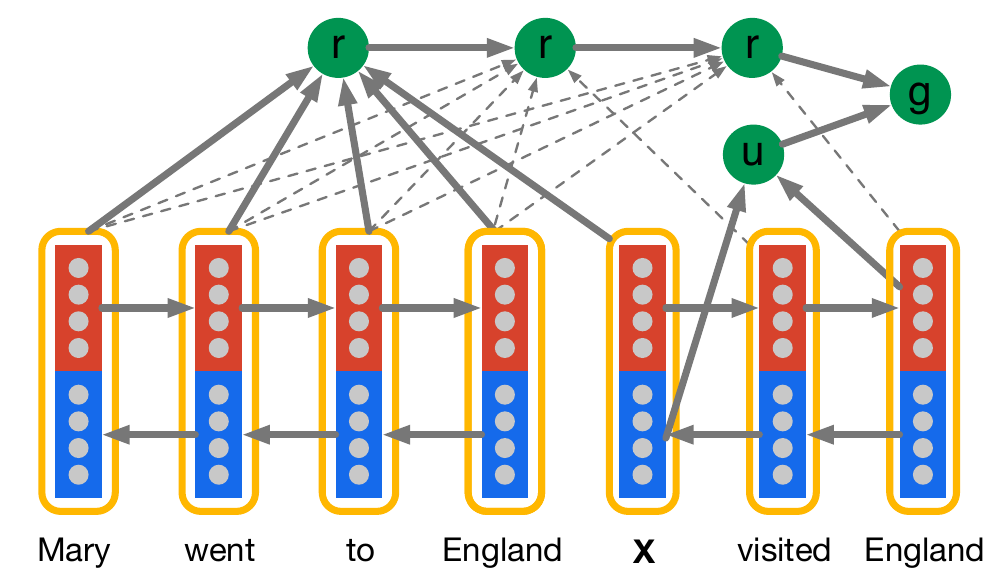
\includegraphics[width=\textwidth]{teachingImpatientReader}
  \caption{Le lecteur impatient prends la requête \textit{X visited England} afin de faire une recherche dans le texte \textit{Mary went to England}, à l’aide du mécanisme d’attention lequel est ici dénoté \texttt{r}, assisté de la requête \texttt{u} \cite{readNcomprehend}}
  \label{fig:teachingImpatientReader}
\end{figure*}

\subsection{Retourner la réponse textuelle sous la forme d'un signal audio}
Une fois une réponse générée, il ne reste plus qu'à la renvoyer à l'utilisateur sous une forme audio, ce qui est un autre calcul rapide qui peut accompli en temps réel. Cela est rendu possible avec le \gls{cnn} \texttt{Wavenet} de \cite{wavenet}. En effet, il est possible de générer n’importe quel ton de voix avec \texttt{Wavenet}, option qui pourrait être laissée à la discrétion de l’utilisateur. À titre d’exemple, cette architecture neurale est tellement puissante qu’il est possible de lui faire imiter la voix du président. Cette découverte récente par \textbf{Google} marquera donc la première occurrence d'une réplique parfaite du timbre d'une voix humaine réelle plutôt qu’une voix aux allures robotiques, ainsi l’illusion est bien réussie. La façon dont \texttt{Wavenet} fonctionne est d’établir un préalable statistique (une variable conditionnée) qui est donné à un premier algorithme qui s’occupe de trouver les bons tons de voix à générer avec \texttt{Wavenet}, à partir du texte. C’est ainsi que \texttt{Wavenet}, conditionné par le ton de voix demandé et par le texte fourni, peut générer la voix de façon réaliste. C’est une méthode point par point, où chaque point dans la vague audio est généré en fonction des points précédents et du conditionnement demandé. L'entraînement de ce réseau se fait à très bas niveau sur le signal qui est à un taux d’échantillonnage de 16 kHz, ce qui est suffisant pour capturer les infimes variations de quelqu’un qui parlerait réellement dans un enregistrement. Cette phase générative est illustrée dans la \autoref{fig:wavenet}.

\begin{figure*}
  \centering
  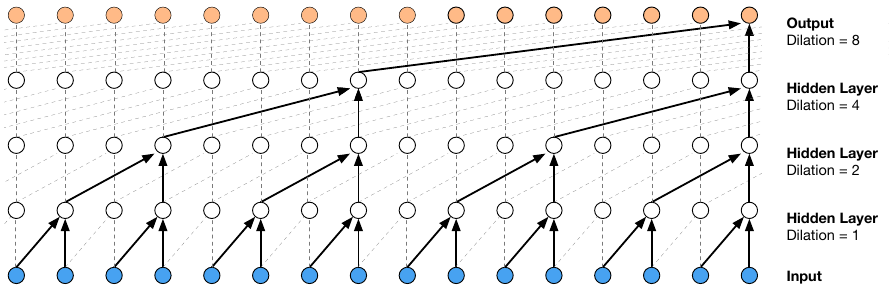
\includegraphics[width=\textwidth]{wavenet}
  \caption{À l’aide de convolutions causales dilatées, il est possible de prédire le prochain point dans la vague audio de façon efficace. Il s'agit d'un modèle autorégressif: les points passés sont utilisés pour prédire les points suivants du même signal. Ainsi, la sortie est remise en entrée pour le calcul de l’étape suivante, cet échantillonngage peut faire usage de mémoire cache, ce qui donne à cet algorithme un temps linéaire pour la génération dépendant de la longueur du signal à générer \cite{wavenet}.}
  \label{fig:wavenet}
\end{figure*}

